% -- Encoding UTF-8 without BOM
% -- XeLaTeX => PDF (BIBER)

\documentclass[]{cv-style}
\sethyphenation[variant=british]{english}{} % Add words between the {} to avoid them to be cut
\usepackage{hyperref}
% \renewcommand{\href}[2]{\href{#1}{\red #2}}

\begin{document}
\header
{Corentin}
{Cadiou}
{PhD student in Astrophysics at Institut d'Astrophysique de Paris (IAP)}
% First name, last name, caption
% \lastupdated

%----------------------------------------------------------------------------------------
%	SIDEBAR SECTION  -- In the aside, each new line forces a line break
%----------------------------------------------------------------------------------------

\begin{aside}
% \hfill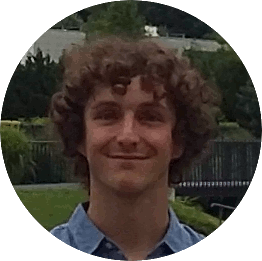
\includegraphics[width=.6\columnwidth]{inset.png}%
% ~
\section{Contact}
72 av. Général Leclerc
75 014 Paris
France
~
+33 6 43 18 66 83
~
Citizenship: French
\href{mailto:corentin.cadiou@iap.fr}{corentin.cadiou@iap.fr}
~
\href{https://cphyc.github.io/}{cphyc.github.io}
\href{https://github.com/cphyc}{
\includegraphics[height=1em]{240px-Octicons-mark-github.png} github.com/cphyc}
%
\section{Science Interests}
\textbf{Astrophysics}
galaxy~formation
cosmic~web
numerical~simulations
cosmology
% 
\section{Languages}
French -- native
English -- fluent (114/120 at TOEFL)
German -- medium
%
\section{Programming}
\textbf{— HPC —}
RAMSES
MPI, OpenMP, Fortran, C++
~
\textbf{— Data analysis —}
yt
Python, NumPy, Linux
~
\textbf{— General skills —}
Linux, bash, javascript
\LaTeX
%
\end{aside}

%----------------------------------------------------------------------------------------
%	EDUCATION SECTION
% ----------------------------------------------------------------------------------------

\section{Education}

\begin{entrylist}
%------------------------------------------------
\entry
{2016--2019}
{PhD in Astrophysics}
{Sorbonne Université \& IAP, Paris France}
{Defense expected in September 2019.}
%------------------------------------------------
\entry
{2015--2016}
{Master's degree in Astrophysics}
{IAP, Paris Observatory \& École Normale Supérieure (ENS), France}
{Specialization in cosmology and numerical astrophysics, \italica{summa cum laude}.}

%------------------------------------------------
\entry
{2015}
{Diploma of the ENS}
{ENS, Paris, France}
{Physics and Computer Sciences.}

%------------------------------------------------
\entryshort
{2012--2014}
{Bachelor's degree, Physics}
{ENS, Paris, France}
%------------------------------------------------
\entryshortnohl
{2012}
{Admitted to the ENS (most selective higher education school in France), \italica{summa cum laude}.}
{}
%------------------------------------------------
\entrynohl
{2010--2012}
{Preparatory school in PCSI/PC*}
{Lycée Sainte-Geneviève, Versailles, France}
{Two-year intensive program in advanced mathematics and physics to prepare the national competitive exam
for entry to engineering schools. Equivalent to two years of Bachelor's degree, \italica{magna cum laude}.
}
%------------------------------------------------
\entryshortnohl
{2010}
{French Baccalauréat (High school diploma), \italica{summa cum laude}}
{Saverne, France}

\end{entrylist}

%----------------------------------------------------------------------------------------
%	RESEARCH SECTION
% ----------------------------------------------------------------------------------------

\section{Research experience}
\begin{entrylist}
%------------------------------------------------
\entry
{2016--2018}
{Member of the project SPIN(E)}
{Agence Nationale de la Recherche (ANR), France}
{ Funded by the French ANR (PI : C.~Pichon).}
%------------------------------------------------
\entry
{2016--2019}
{Post-graduate research}
{IAP, Paris, France}
{``The Origin of the Hubble Sequence'' supervisors: Christophe Pichon and Yohan Dubois, funded by the ENS.}
%------------------------------------------------
\entry
{2016}
{Kavli Summer Program in Astrophysics}
{UCSC, California, USA}
{``Evolution of the atmosphere of close-by Kepler exoplanets'', supervisors: James Owen and Fred Adams.}
%-----------------------------------------------
\entry
{2014}
{Research internship}
{UCSC, California, USA}
{``Angular momentum mixing processes in red giants to explain
  the slow-rotating cores problem'', supervisor: Pascale Garaud.}
\end{entrylist}

%----------------------------------------------------------------------------------------
%	AWARDS SECTION
%----------------------------------------------------------------------------------------
\section{Awards}
\begin{entrylist}
%------------------------------------------------
\entry
{2018}
{NumFOCUS New Contributor Award}
{}
{Awarded for developing and extending the RAMSES frontend of the yt project, a Python package for analyzing and visualizing astrophysical simulations.}
% ------------------------------------------------
\entry
{2017--now}
{yt team member}
{}
{Nominated for continuous and significant contributions to the yt project.}
% ------------------------------------------------
\entry
{2016--2019}
{ILP fellowship}
{}
{5000€ grant per annum for research expenses, including travel.}
% ------------------------------------------------
\entry
{2012--2019}
{ENS scholarship \& ENS doctoral fellowship}
{}
{Prestigious full stipend awarded nationwide to 20 fellows.}
\end{entrylist}

%----------------------------------------------------------------------------------------
%	PUBLICATION SECTION
%----------------------------------------------------------------------------------------
\newpage
\section{Publications}
% My work focuses on the link between galaxy formation and the large scale structures of the Universe (the ``cosmic web'') using numerical simulations and theory.

\begin{entrylist}
%------------------------------------------------
\entry
{2018}
{Accurate tracer particles of the baryons dynamics in the adaptive mesh refinement code Ramses}
{Submitted to A\&A}
{\textbf{C.~Cadiou}, Y.~Dubois \& C.~Pichon, \href{http://adsabs.harvard.edu/cgi-bin/bib_query?arXiv:1810.11401}{arXiv:1810.11401}\\ % TODO: arxiv link ASAP
  {\bf About:} A new numerical method to track the accretion of baryons onto galaxies.\\
  {\bf Contribution:} Main author.
}
%------------------------------------------------
\entry
{2018}
{Galaxies flowing in the oriented saddle frame of the cosmic web}
{Submitted to MNRAS}
{K.~Kraljic, C.~Pichon, Y.~Dubois, S.~Codis, \textbf{C.~Cadiou}, et al., \href{http://adsabs.harvard.edu/cgi-bin/bib_query?arXiv:1810.05211}{arXiv:1810.05211}.\\
  {\bf About:} The effect of the cosmic web on galaxy formation in numerical simulations.\\
  {\bf Contribution:} Co-author of the theory section.
}
%------------------------------------------------
\entry
{2017}
{Galaxy evolution in the metric of the Cosmic Web}
{MNRAS}
{K.~Kraljic, S.~Arnouts, C.~Pichon, C.~Laigle, S.~de~la~Torre,
  D.~Vibert, \textbf{C.~Cadiou}, et al., \href{http://adsabs.harvard.edu/cgi-bin/bib_query?arXiv:1710.02676}{arXiv:1710.02676}\\
  {\bf About:} The effect of the cosmic web on galaxy formation in observations.\\
  {\bf Contribution:} Provided theory part.
}
%------------------------------------------------
\entry
{2017}
{How does the cosmic web impact assembly bias?}
{MNRAS}
{M.~Musso, \textbf{C.~Cadiou}, C.~Pichon, S. Codis, K.~Kraljic  \& Y.~Dubois,
  \href{http://adsabs.harvard.edu/cgi-bin/bib_query?arXiv:1709.00834}{arXiv:1709.00834}\\
  {\bf About:} The effect of the cosmic web on dark matter halo formation, theoretical.\\
  {\bf Contribution:} Co-author of the paper.
}
\end{entrylist}

% ----------------------------------------------------------------------------------------
% 	TALKS SECTION
% ----------------------------------------------------------------------------------------
% \newpage
\section{Talks and Posters}

\textbf{Seminars and workshops}

\begin{entrylist}
% ------------------------------------------------
\entryshortnohl{Sept. 2016}
{Ramses User Meeting}
{Lyon, France}
% ------------------------------------------------
\entryshortnohl{May 2017}
{CITA journal club}
{Toronto, Canada}
% ------------------------------------------------
\entryshortnohl{Sept. 2017}
{Ramses User Meeting}
{Nice, France}
% ------------------------------------------------
\entryshortnohl{Sept. 2017}
{SPIN(E) ANR Meeting}
{Agay, France}
% ------------------------------------------------
\entryshortnohl{Nov. 2017}
{KIAS journal club}
{Seoul, South Korea}
% ------------------------------------------------
\entryshortnohl{April 2018}
{CRAL journal club}
{Lyon, France}
% ------------------------------------------------
\entryshortnohl{May. 2018}
{SPIN(E) ANR Meeting}
{Edinburgh, UK}
% ------------------------------------------------
\entryshortnohl{Sept. 2018}
{West Coast Swings workshop}
{Perth, Australia}
% ------------------------------------------------
\end{entrylist}


\textbf{Internal seminars}

\begin{entrylist}
\entryshortnohl{2016, 2017}
{ED127 PhD day}
{Paris, France}
% ------------------------------------------------
\entryshortnohl{2016, 2017}
{IAP PhD day}
{Paris, France}
% ------------------------------------------------
\entryshortnohl{2016, 2017}
{YMCA, IAP student seminar}
{Paris, France}
\end{entrylist}


\textbf{Posters}

\begin{entrylist}
\entryshortnohl{Sept. 2018}
{Analytics, Computation and Inference in Cosmology}
{Cargese, France}
% ------------------------------------------------
\entryshortnohl{Oct. 2018}
{Highlights \& prospects for numerical astrophysics in France (Astrosim)}
{Lyon, France}

\end{entrylist}

%----------------------------------------------------------------------------------------
%    TEACHING SECTION
%----------------------------------------------------------------------------------------
\section{Teaching}
\begin{entrylist}
%------------------------------------------------
\entry
{2016--2019}
{Teaching Assistant}
{Sorbonne Université, Paris, France}
{Courses included: concept and methods of Physics at B.Sc. level (192 hours). Graded all written work, oral and final written exams and assisted with labs.}
\end{entrylist}

%----------------------------------------------------------------------------------------
%    RESPONSIBILITIES + OUTREACH SECTION
%----------------------------------------------------------------------------------------
\newpage
\section{Responsibilities and outreach}
\begin{entrylist}
%------------------------------------------------
\entrynohl
{2016--2017}
{Organizer of the IAP pre-seminar.}
{}
{Weekly meeting with the invited speaker with all the PhD students.}
%------------------------------------------------
\entrynohl
{2018}
{Organizer of the ``Mystery Science Picture'' (MSciPic)}
{}
{Monthly release of a scientific picture for public outreach for the Société Française de Physique (SFP).}
%------------------------------------------------
\entrynohl
{2017--2019}
{Journée de la Science (Open House day)}
{}
{Yearly public outreach event about general astronomy at IAP and Sorbonne Université.}
\end{entrylist}

%----------------------------------------------------------------------------------------
%	OTHER EXPERIENCE SECTION
% ----------------------------------------------------------------------------------------

\section{Other Experiences}

\begin{entrylist}
%------------------------------------------------
\entrynohl
{2015}
{6-months internship in an IT company}
{Linagora, Paris, France}
{Development of a real-time peer-to-peer collaborative text editor.}

\vspace{1em}

%------------------------------------------------
\entryshortnohl
{2015}
{Ranked 2/130th team at the \textbf{Google Hashcode} programming competition.}
{Paris, France}

%------------------------------------------------
\entryshortnohl
{2012--2013}
{Team member of the ENS student association.}
{Paris, France}

\entryshortnohl
{2008--now}
{Member of the BECD (Bénin Europe Coopération et Développement) an NGO to foster development in Benin.}
{France \& Benin}

%------------------------------------------------
\end{entrylist}


\end{document}

% Local Variables:
% TeX-engine: xetex
% End:
